\chapter{Abkürzungsverzeichnis}

\begin{acronym}
	\acro{maui}[MAUI]{Multiplatform App UI}
	\acro{owin}[OWIN]{Open Web Interface}
	\acro{wpf}[WPF]{Windows Presentation Foundation}
	\acro{vb6}[VB6]{Visual Basic 6}
	\acro{http}[HTTP]{Hypertext Transfer Protocol}
	\acro{gui}[GUI]{Graphical User Interface}
	\acro{ava}[AVA]{Ausschreibung Vergabe Abrechnung}
	\acro{hoai}[HOAI]{Verordnung über die Honorare für Architekten- und Ingenieurleistungen}
	\acro{bim}[BIM]{Building Information Modeling}
\end{acronym}

\clearpage

\chapter{Abbildungsverzeichnis}

\begin{figure}[H]
	\centering
	{\caption{Baumstruktur eines Leistungsverzeichnisses in der ORCA \ac{ava}}
		\label{fig:LV-der-AVA}}
	{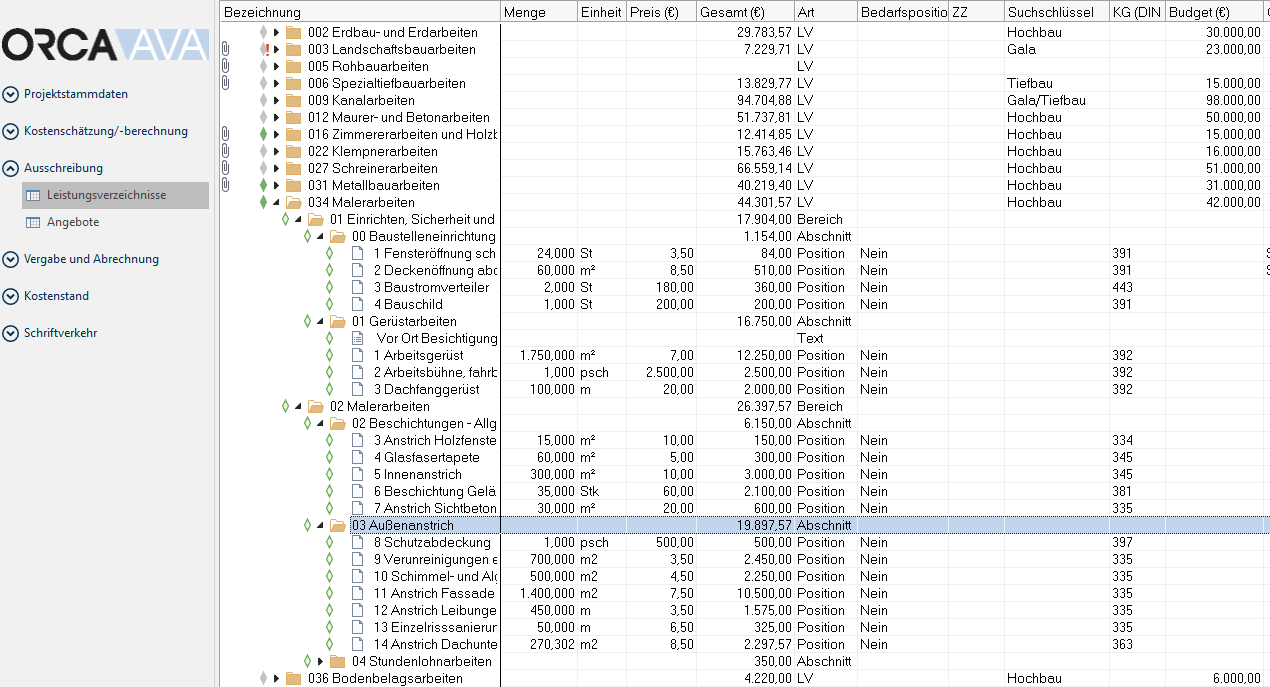
\includegraphics[width=1\textwidth]{\figdir/orca-ava-tree}}
\end{figure}

\begin{figure}[H]
	\centering
	{\caption{Baumstruktur eines Leistungsverzeichnisses im implementierten TreeList-Control}
		\label{fig:tree-result}}
	{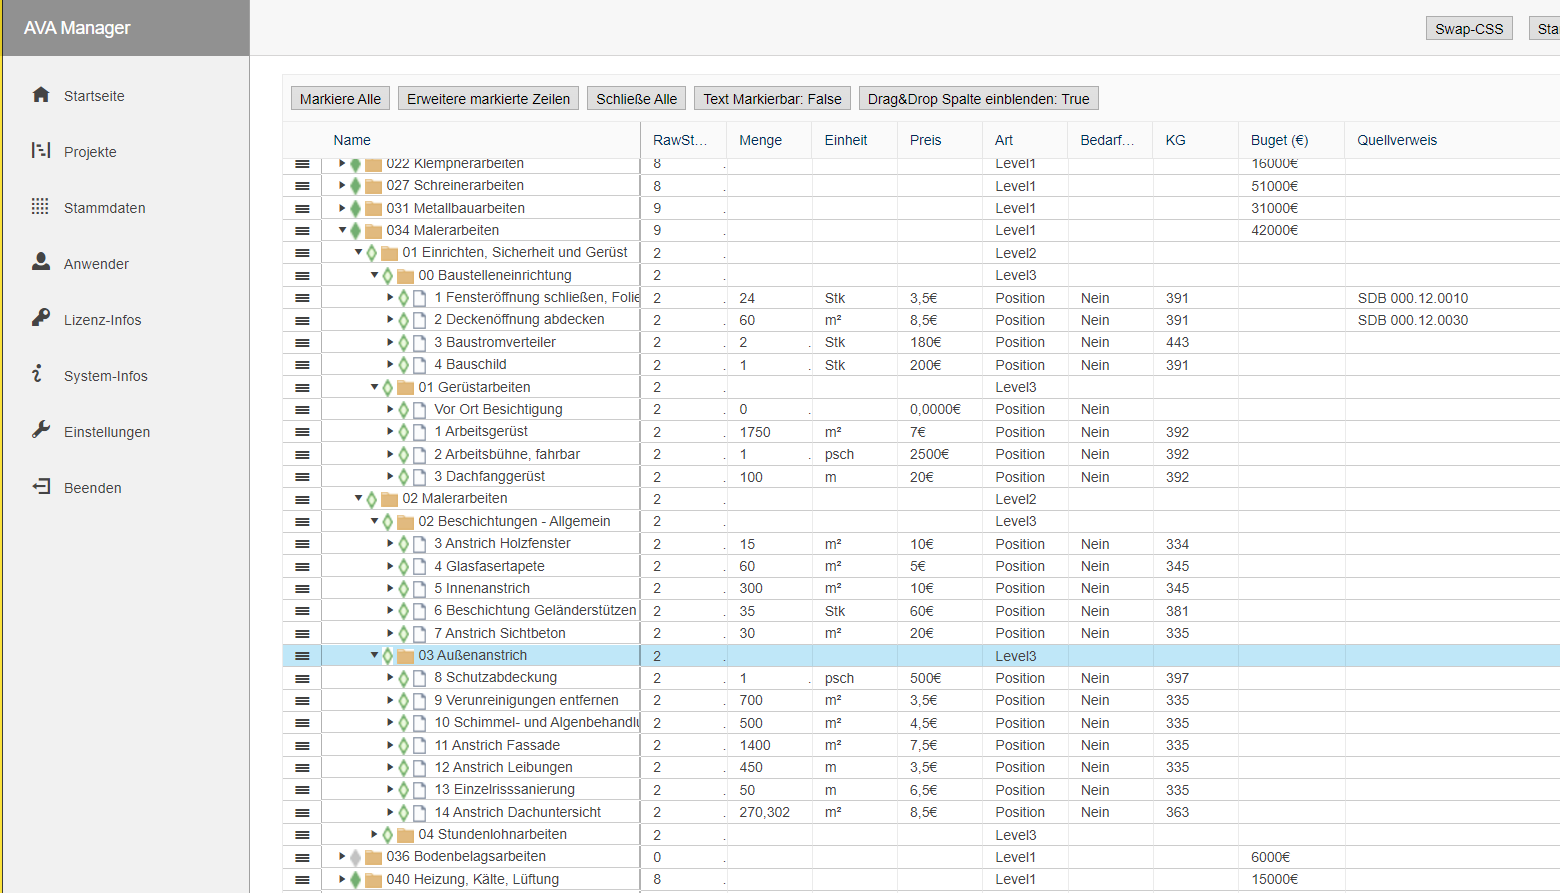
\includegraphics[width=1\textwidth]{\figdir/tree-result}}
\end{figure}


%%% Local Variables: 
%%% mode: latex
%%% TeX-master: "thesis.tex"
%%% End: 
